\documentclass[../../main.tex]{subfiles}
\begin{document}
\section{Validity of a Two-dimensional beam} \label{sec:validity-of-a-2d-beam}
This section is an extention of section \ref{sec:validity-of-a-cantilever-timoshenko-beam} and the article \cite{LVV09}. As seen in the previous section, the two-dimensional model does have some characteristics that are not related to beam-type problems. This is also true for the three-dimensional model. 

The results in this section will show that the three-dimensional model has a lot of non-beam type eigenvalues. It is due to this reason, the authors of \cite{LVV09} suggested to use the two-dimensional model as an intermediate step. The the previous section, the validity of a cantilever Timoshenko beam was investigated using a cantilever two-dimensional beam as a reference. In this section, the validity of a cantilever two-dimensional beam will be investigated using a cantilever three-dimensional beam as a reference.

\subsection{The models}
The two-dimensional model is the same model as used in the previous section, Problem T-2 defined in section \ref{ssec:2D_Model:ModelProblem}. From section \ref{ssec:3D_Model:ModelProblems}, the cantilever three-dimensional model, referred to as Problem 3D-1.

Figure \ref{fig:2Dv3D} shows the two beams side-by-side.

\FloatBarrier
\begin{figure}[h!]
	\scalebox{.8}{
		\makebox[\textwidth][c]{
			\caption{Side-by-side comparison of the beams.}
			\label{fig:2Dv3D}
			\centering
			\begin{minipage}[b]{0.7\linewidth}
				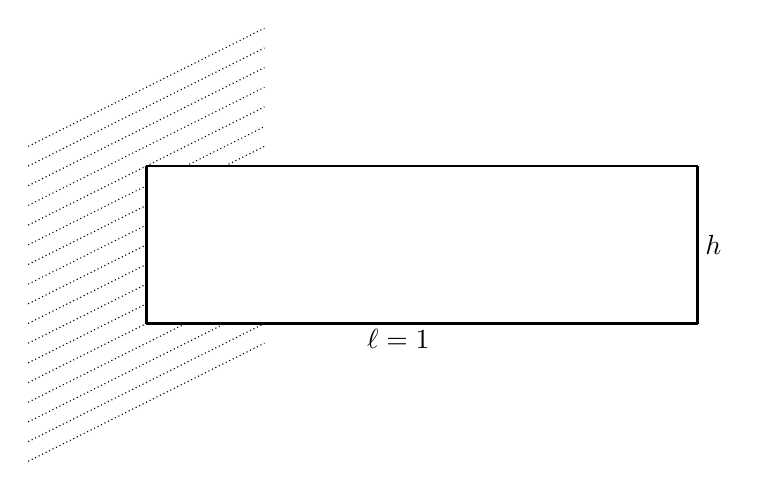
\begin{tikzpicture}
					\draw[line width = 0.3mm] (0,1) -- (7,1);
					\draw[line width = 0.3mm] (0,-1) -- (7,-1);
					\draw[line width = 0.3mm] (7,-1) -- (7,1);
					\draw[line width = 0.3mm] (0,-1) -- (0,1);
					
					
					\draw[scale=0.5, domain=-3:3, smooth, variable=\x,densely dotted] plot ({\x}, {0.5*\x+4});
					\draw[scale=0.5, domain=-3:3, smooth, variable=\x,densely dotted] plot ({\x}, {0.5*\x+3.5});
					\draw[scale=0.5, domain=-3:3, smooth, variable=\x,densely dotted] plot ({\x}, {0.5*\x+3});
					\draw[scale=0.5, domain=-3:3, smooth, variable=\x,densely dotted] plot ({\x}, {0.5*\x+2.5});
					\draw[scale=0.5, domain=-3:3, smooth, variable=\x,densely dotted] plot ({\x}, {0.5*\x+2});
					
					\draw[scale=0.5, domain=-3:0, smooth, variable=\x,densely dotted] plot ({\x}, {0.5*\x+1.5});
					\draw[scale=0.5, domain=-3:0, smooth, variable=\x,densely dotted] plot ({\x}, {0.5*\x+1});
					
					
					\draw[scale=0.5, domain=1:3, smooth, variable=\x,densely dotted] plot ({\x}, {0.5*\x+1.5});
					\draw[scale=0.5, domain=2:3, smooth, variable=\x,densely dotted] plot ({\x}, {0.5*\x+1});
					
					\draw[scale=0.5, domain=-3:0, smooth, variable=\x,densely dotted] plot ({\x}, {0.5*\x+0.5});
					\draw[scale=0.5, domain=-3:0, smooth, variable=\x,densely dotted] plot ({\x}, {0.5*\x});
					\draw[scale=0.5, domain=-3:0, smooth, variable=\x,densely dotted] plot ({\x}, {0.5*\x-0.5});
					\draw[scale=0.5, domain=-3:0, smooth, variable=\x,densely dotted] plot ({\x}, {0.5*\x-1});
					\draw[scale=0.5, domain=-3:0, smooth, variable=\x,densely dotted] plot ({\x}, {0.5*\x-1.5});
					\draw[scale=0.5, domain=-3:0, smooth, variable=\x,densely dotted] plot ({\x}, {0.5*\x-2});
					\draw[scale=0.5, domain=-3:1, smooth, variable=\x,densely dotted] plot ({\x}, {0.5*\x-2.5});
					\draw[scale=0.5, domain=-3:2, smooth, variable=\x,densely dotted] plot ({\x}, {0.5*\x-3});
					\draw[scale=0.5, domain=-3:3, smooth, variable=\x,densely dotted] plot ({\x}, {0.5*\x-3.5});
					\draw[scale=0.5, domain=-3:3, smooth, variable=\x,densely dotted] plot ({\x}, {0.5*\x-4});
					
					\node at (7.2,0) {$h$};
					\node at (3.2,-1.2) {$\ell = 1$};
				\end{tikzpicture}
				\subcaption{Two-Dimensional Elastic Body}
			\end{minipage}
			\begin{minipage}[b]{0.7\linewidth}
				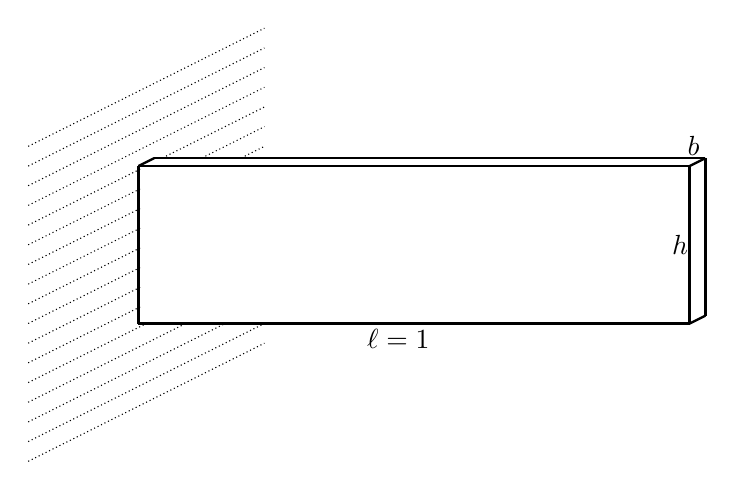
\begin{tikzpicture}
					\draw[line width = 0.3mm] (-0.1,1) -- (6.9,1);
					\draw[line width = 0.3mm] (-0.1,-1) -- (6.9,-1);
					\draw[line width = 0.3mm] (6.9,-1) -- (6.9,1);
					\draw[line width = 0.3mm] (-0.1,-1) -- (-0.1,1);
					
					\draw[line width = 0.3mm] (0.1,1.1) -- (7.1,1.1);
					\draw[line width = 0.3mm] (7.1,-0.9) -- (7.1,1.1);
					
					\draw[line width = 0.3mm] (-0.1,1) -- (0.1,1.1);
					\draw[line width = 0.3mm] (6.9,1) -- (7.1,1.1);
					\draw[line width = 0.3mm] (6.9,-1) -- (7.1,-0.9);
					
					
					
					\draw[scale=0.5, domain=-3:3, smooth, variable=\x,densely dotted] plot ({\x}, {0.5*\x+4});
					\draw[scale=0.5, domain=-3:3, smooth, variable=\x,densely dotted] plot ({\x}, {0.5*\x+3.5});
					\draw[scale=0.5, domain=-3:3, smooth, variable=\x,densely dotted] plot ({\x}, {0.5*\x+3});
					\draw[scale=0.5, domain=-3:3, smooth, variable=\x,densely dotted] plot ({\x}, {0.5*\x+2.5});
					
					\draw[scale=0.5, domain=-3:-0.1, smooth, variable=\x,densely dotted] plot ({\x}, {0.5*\x+2});
					\draw[scale=0.5, domain=-3:-0.1, smooth, variable=\x,densely dotted] plot ({\x}, {0.5*\x+1.5});
					\draw[scale=0.5, domain=-3:-0.1, smooth, variable=\x,densely dotted] plot ({\x}, {0.5*\x+1});
					
					\draw[scale=0.5, domain=0.5:3, smooth, variable=\x,densely dotted] plot ({\x}, {0.5*\x+2});
					\draw[scale=0.5, domain=1.5:3, smooth, variable=\x,densely dotted] plot ({\x}, {0.5*\x+1.5});
					\draw[scale=0.5, domain=2.5:3, smooth, variable=\x,densely dotted] plot ({\x}, {0.5*\x+1});
					
					\draw[scale=0.5, domain=-3:-0.1, smooth, variable=\x,densely dotted] plot ({\x}, {0.5*\x+0.5});
					\draw[scale=0.5, domain=-3:-0.1, smooth, variable=\x,densely dotted] plot ({\x}, {0.5*\x});
					\draw[scale=0.5, domain=-3:-0.1, smooth, variable=\x,densely dotted] plot ({\x}, {0.5*\x-0.5});
					\draw[scale=0.5, domain=-3:-0.1, smooth, variable=\x,densely dotted] plot ({\x}, {0.5*\x-1});
					\draw[scale=0.5, domain=-3:-0.1, smooth, variable=\x,densely dotted] plot ({\x}, {0.5*\x-1.5});
					\draw[scale=0.5, domain=-3:0, smooth, variable=\x,densely dotted] plot ({\x}, {0.5*\x-2});
					\draw[scale=0.5, domain=-3:1, smooth, variable=\x,densely dotted] plot ({\x}, {0.5*\x-2.5});
					\draw[scale=0.5, domain=-3:2, smooth, variable=\x,densely dotted] plot ({\x}, {0.5*\x-3});
					\draw[scale=0.5, domain=-3:3, smooth, variable=\x,densely dotted] plot ({\x}, {0.5*\x-3.5});
					\draw[scale=0.5, domain=-3:3, smooth, variable=\x,densely dotted] plot ({\x}, {0.5*\x-4});
					
					\node at (6.95,1.25) {$b$};
					\node at (6.78,0) {$h$};
					\node at (3.2,-1.2) {$\ell = 1$};
					

				\end{tikzpicture}
				\subcaption{Three-Dimensional Elastic Body}
				
			\end{minipage}
		}
	}
\end{figure}
\FloatBarrier

\subsection{Calculating the eigenvalues}
Similar to calculating the eigenvalues of the two-dimensional beam, to calculate the eigenvalues of the three-dimensional beam, the Finite Element Method is used. In section \ref{sec:FEM:3D}, the Finite Element Method for the three-dimensional beam is derived. Section \ref{3dFEM_EP} gives the following eigenvalue problem for the three-dimensional beam:

\subsubsection{Problem 2D-1E}
Find a real number $\lambda$ and a function $\bar{u} \in S^h$ such that
\begin{eqnarray}
	K\bar{u} & = & M\lambda{\bar{u}},
\end{eqnarray} where $K$ and $M$ are the standard Finite Element Method matrices for bi-cubic basis functions. The definition of the matrices are given in section \ref{sec:FEM:2D}.

\subsubsection{Problem 3D-1E}
Find a real number $\lambda$ and a function $\bar{u} \in S^h$ such that
\begin{eqnarray}
	K\bar{u} & = & M\lambda{\bar{u}},
\end{eqnarray} where $K$ and $M$ are the standard Finite Element Method matrices for tri-cubic basis functions. The definition of the matrices are given in section \ref{sec:FEM:3D}.

\subsubsection{Accuracy of the eigenvalues}
Figure \ref{fig:conv_3d_eig} show the rate of convergence of the first 20 eigenvalues of Problem 3D-1E. 

\begin{figure}[H]
    \centering
    \begin{adjustbox}{center}
        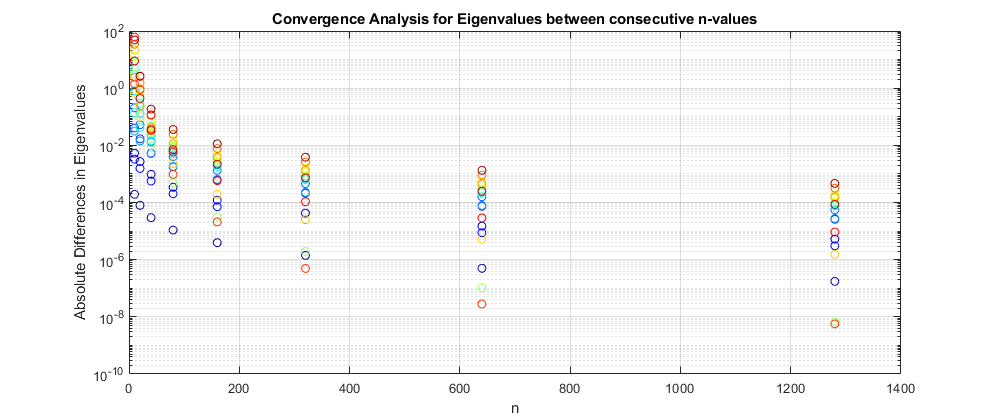
\includegraphics[scale=0.7]{Convergence.png}
    \end{adjustbox}
    \caption{Rate of convergence of the first 20 eigenvalues.}
    \label{fig:conv_3d_eig}
\end{figure}
\textcolor{red}{Update this figure.}

Similar to the two-dimensional case, the number of elements can be chosen so that at least the first 10 eigenvalues are accurate to 5 significant digits.

\subsection{Comparing the mode shapes}
The method to match up the eigenvalues remains the same as in the previous section. Since the three-dimensional model is more complex, there are more mode shapes that do no appear in the Timoshenko model or two-dimensional model. The focus remains on beam-type problems, so the mode shapes relating to beam type problems are most important.

\subsubsection{Mode shapes relating to beam type eigenvalues.}
Figure \ref{fig:beam-2dv3d} show some examples of beam type mode shapes for the displacement $u$.

\begin{figure}[h!]
	\scalebox{.8}{
		\makebox[\textwidth][c]{
			\centering
			\begin{minipage}[b]{0.8\linewidth}
				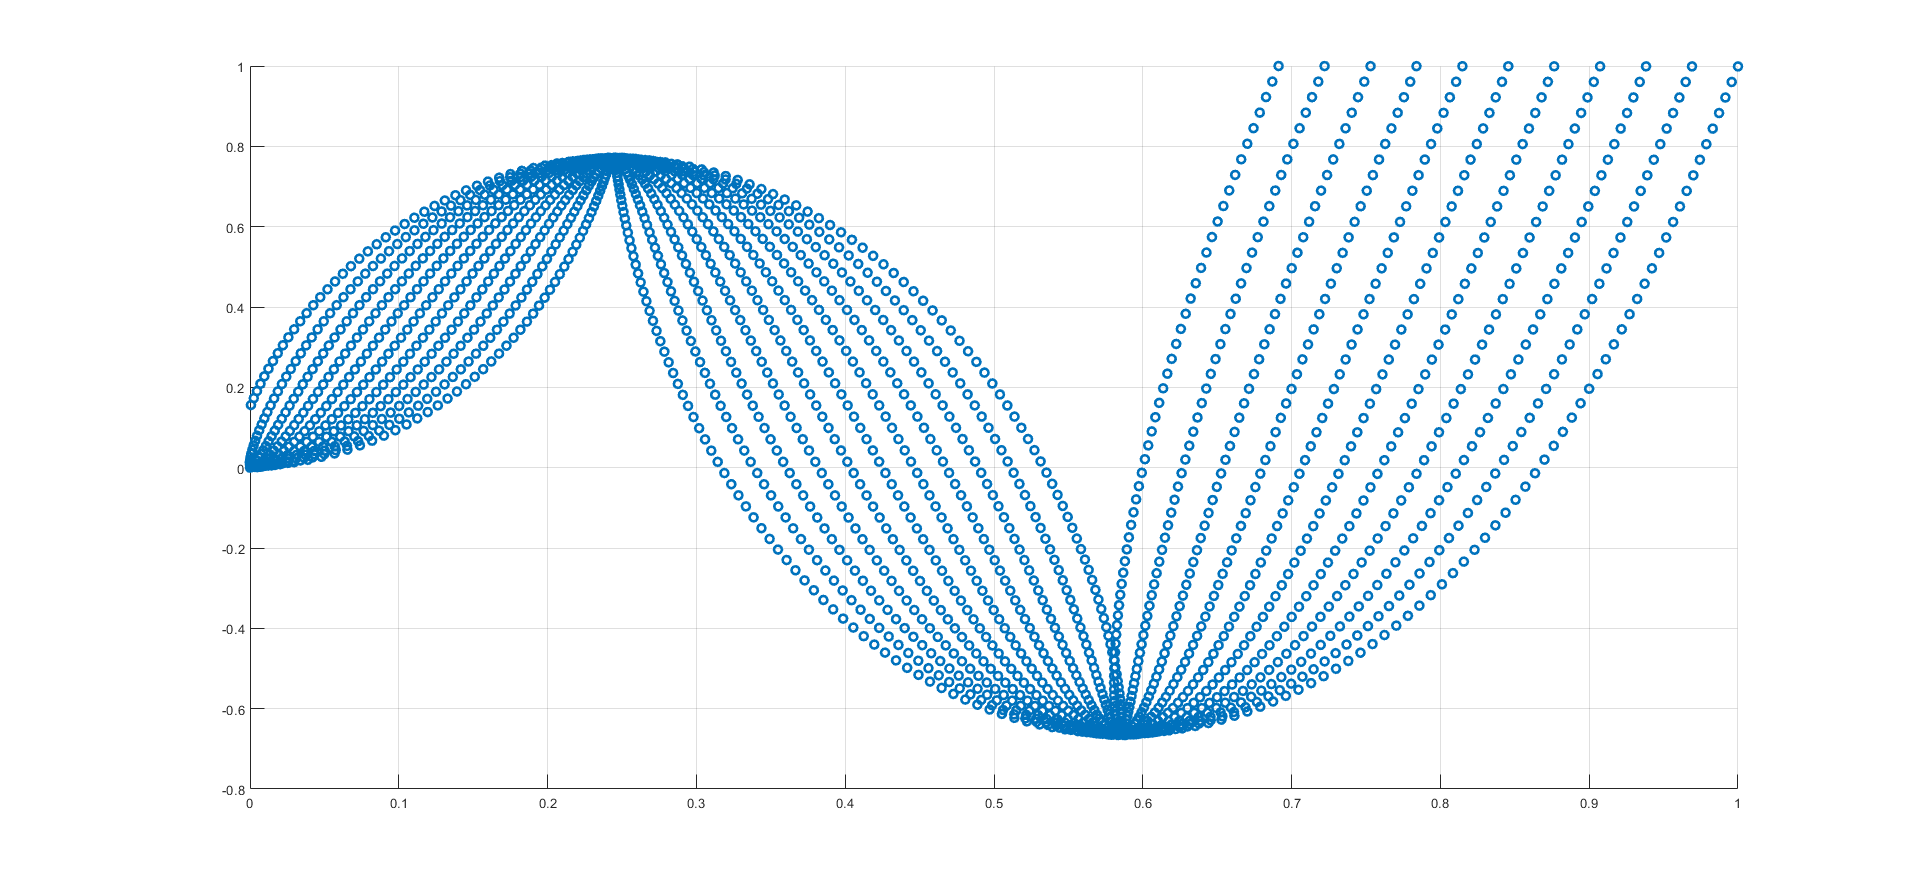
\includegraphics[width=1\linewidth]{3D12.png}
				\subcaption{3D Beam Type - $\lambda_{12} = 2.3293$}
				\label{fig:minipage2}
			\end{minipage}
			\begin{minipage}[b]{0.8\linewidth}
				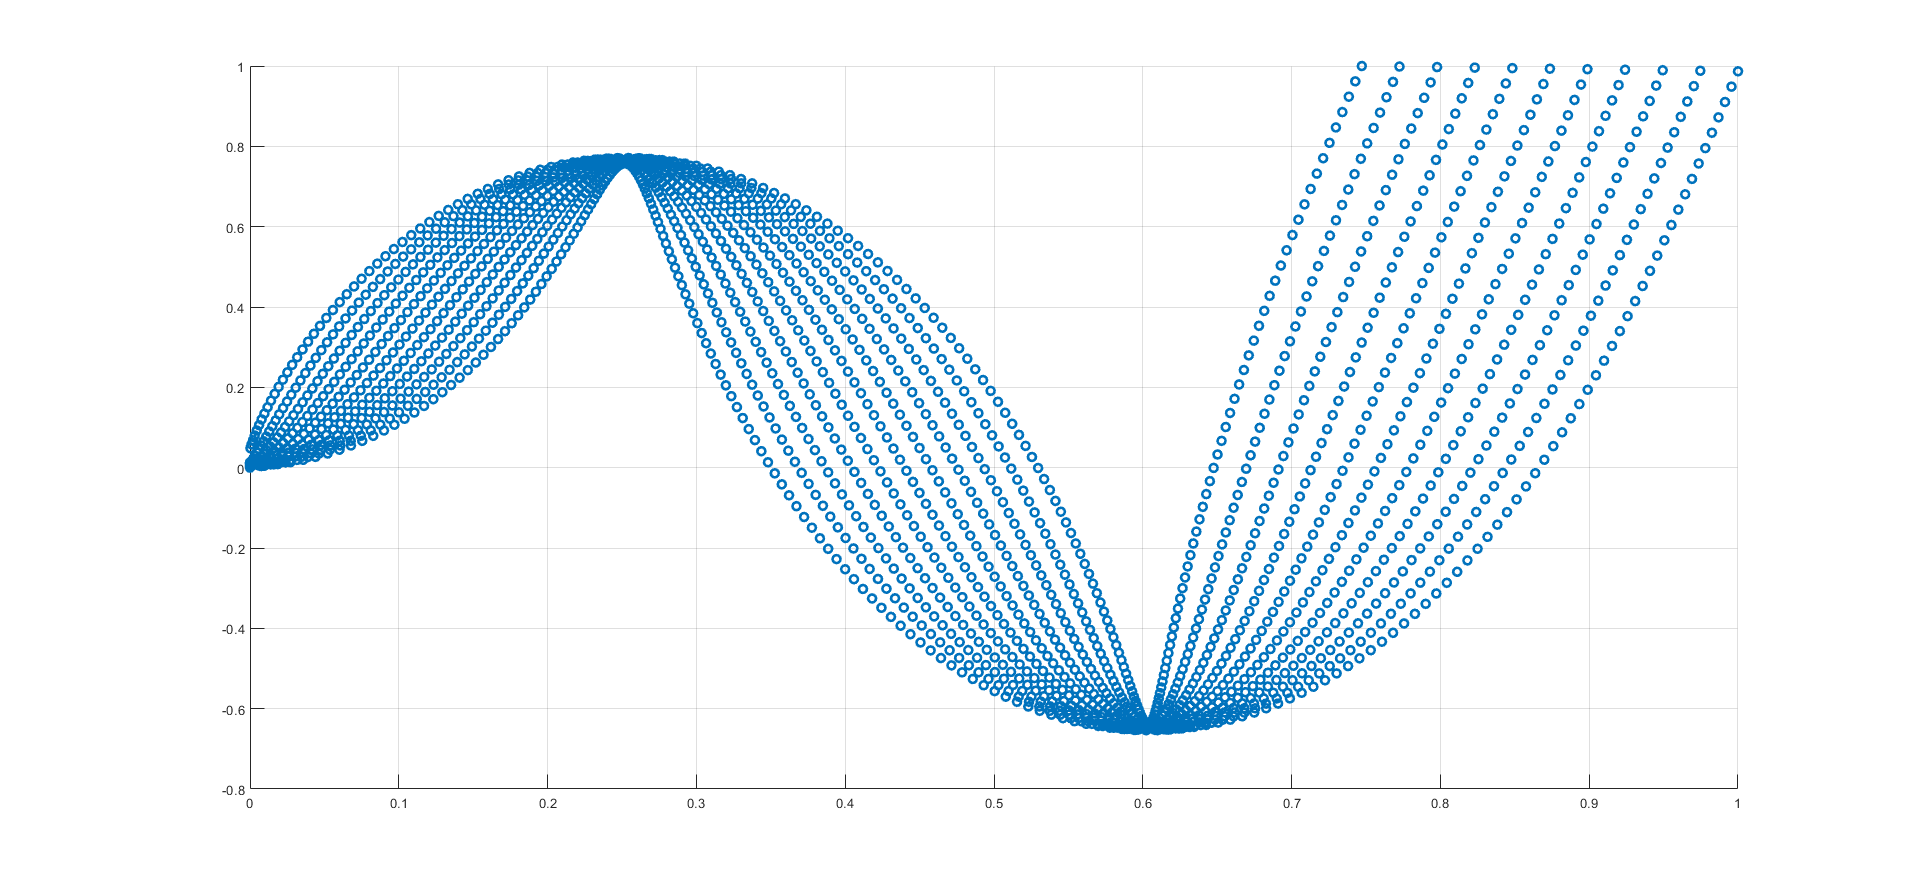
\includegraphics[width=1\linewidth]{2D3.png}
				\subcaption{2D Beam Type - $\lambda_3 = 2.3273$}
				\label{fig:minipage1}
			\end{minipage}
	}}
	\scalebox{.8}{
		\makebox[\textwidth][c]{
			\centering
			\begin{minipage}[b]{0.8\linewidth}
				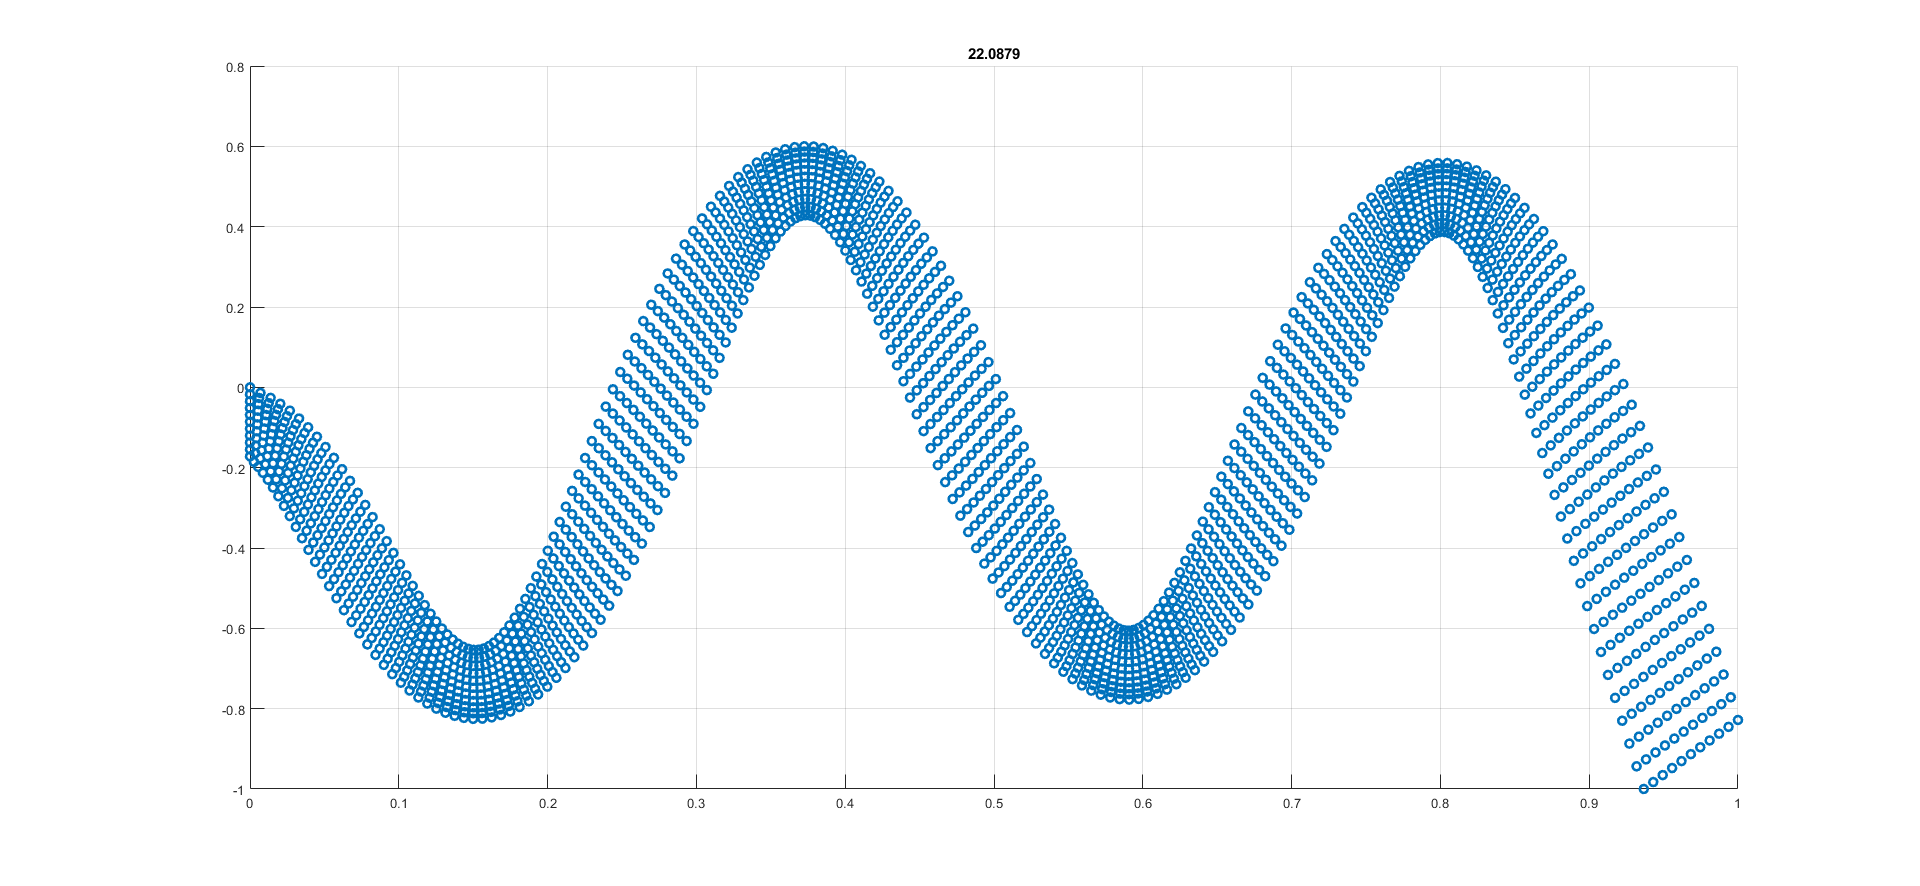
\includegraphics[width=1\linewidth]{3D22.png}
				\subcaption{3D Beam Type - $\lambda_{24} = 21.929$}
				\label{fig:minipage2}
			\end{minipage}
			\begin{minipage}[b]{0.8\linewidth}
				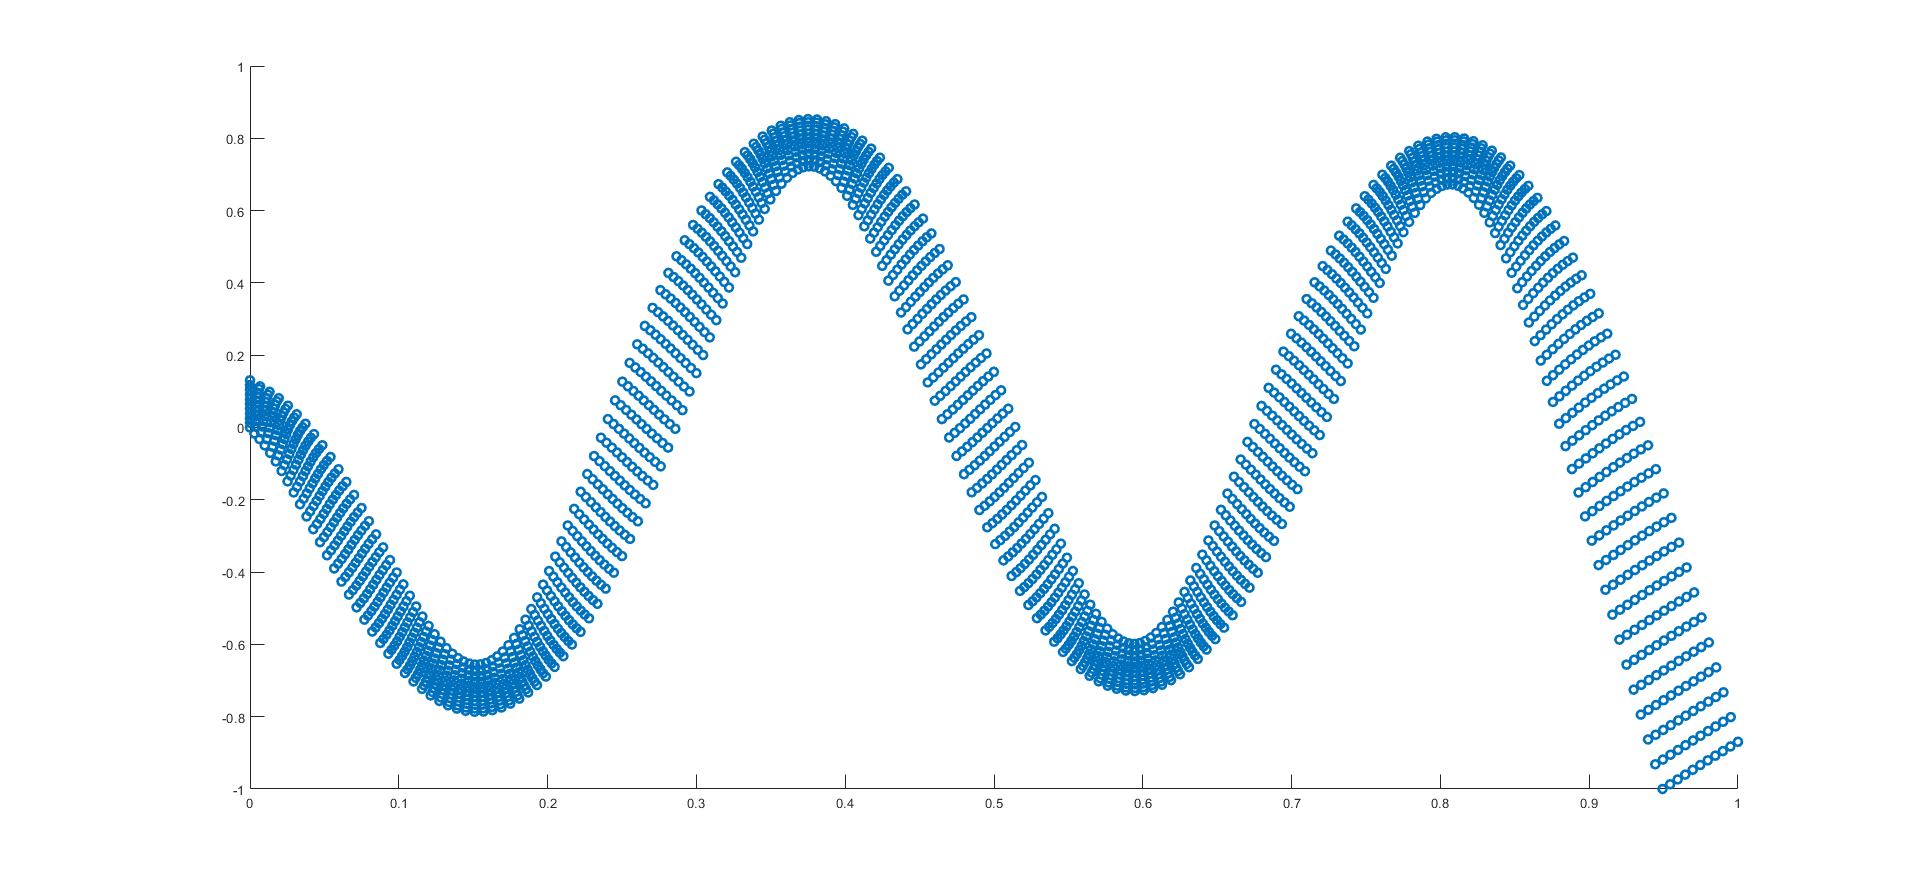
\includegraphics[width=1\linewidth]{2D6.png}
				\subcaption{2D Beam Type - $\lambda_6 = 21.911$}
				\label{fig:minipage1}
			\end{minipage}
			\caption{Mode shapes of the displacement $w$ with $h=1/20$.}
			\label{fig:beam-2dv3d}
	}}
\end{figure}
\FloatBarrier

\subsubsection{Mode shapes relating to non-beam type eigenvalues that are present in the two-dimensional model.}
Figure \ref{fig:nonbeam-2dv3d} show examples of mode shapes relating to non-beam type eigenvalues for the displacement $u$.

\FloatBarrier
\begin{figure}[h!]
	\scalebox{.8}{
		\makebox[\textwidth][c]{
			\centering
			\begin{minipage}[b]{0.8\linewidth}
				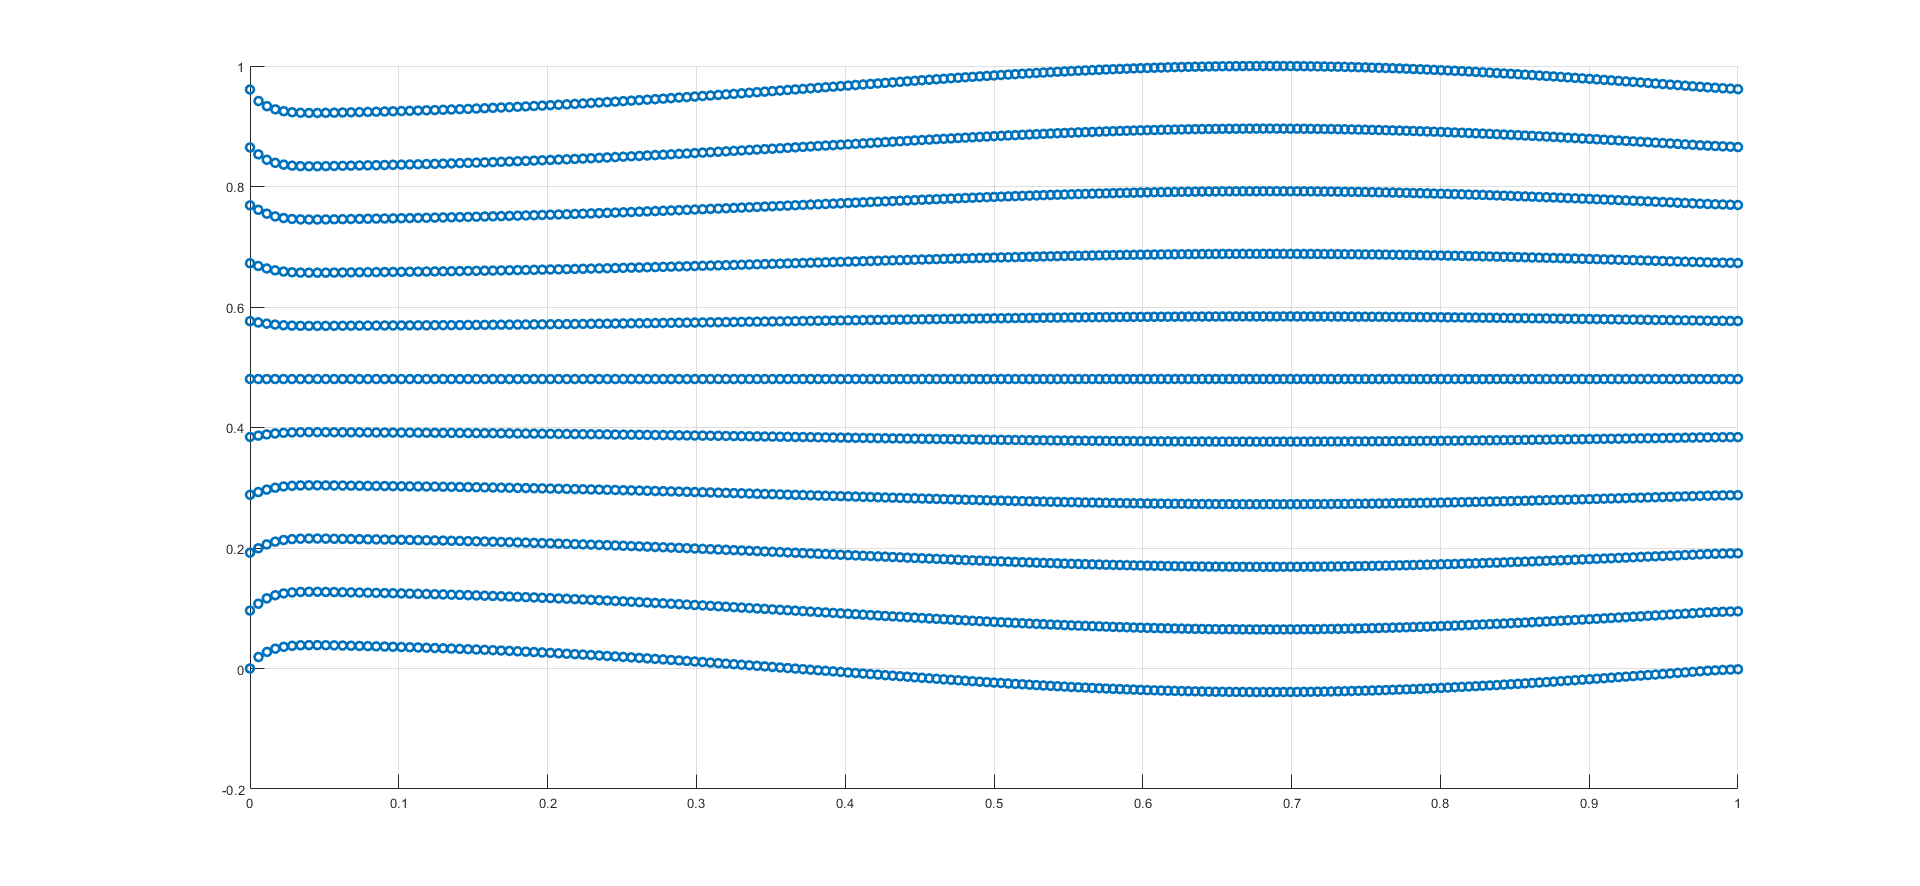
\includegraphics[width=1\linewidth]{3D33.png}
				\subcaption{3D Non-Beam Type - $\lambda_{33} = 69.374$}
				\label{fig:minipage2}
			\end{minipage}
			\begin{minipage}[b]{0.8\linewidth}
				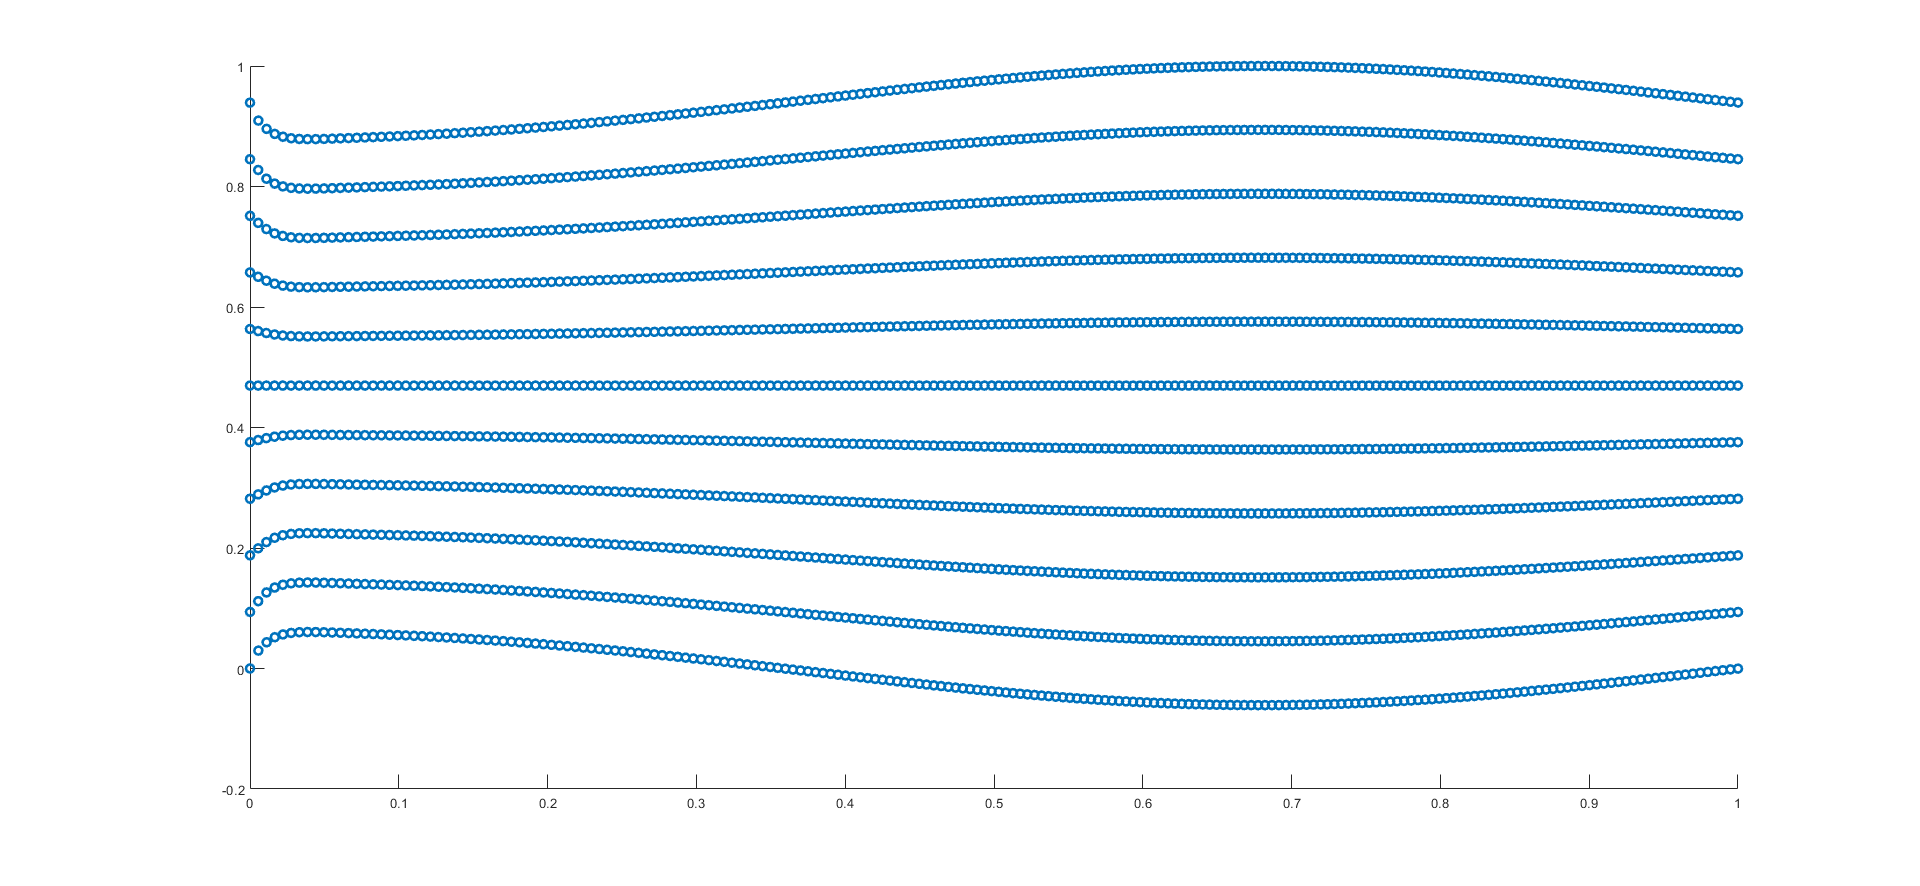
\includegraphics[width=1\linewidth]{2D8.png}
				\subcaption{2D Non-Beam Type - $\lambda_8 = 69.344$}
				\label{fig:minipage1}
			\end{minipage}
			\caption{Mode shapes of the displacement $w$ with $h=1/20$.}
			\label{fig:nonbeam-2dv3d}
	}}
\end{figure}
\FloatBarrier

\subsubsection{Mode shapes relating to non-beam type eigenvalues that are not present in the two-dimensional model.}
Figure \ref{fig:nonbeam-2dv3d} show examples of mode shapes relating to non-beam type eigenvalues for the displacement $u$ which are not present in the two-dimensional model. These mode shapes only appear in the three-dimensional beam.
\FloatBarrier
\begin{figure}[h!]
	\scalebox{.8}{
		\makebox[\textwidth][c]{
			\centering
			\begin{minipage}[b]{0.8\linewidth}
				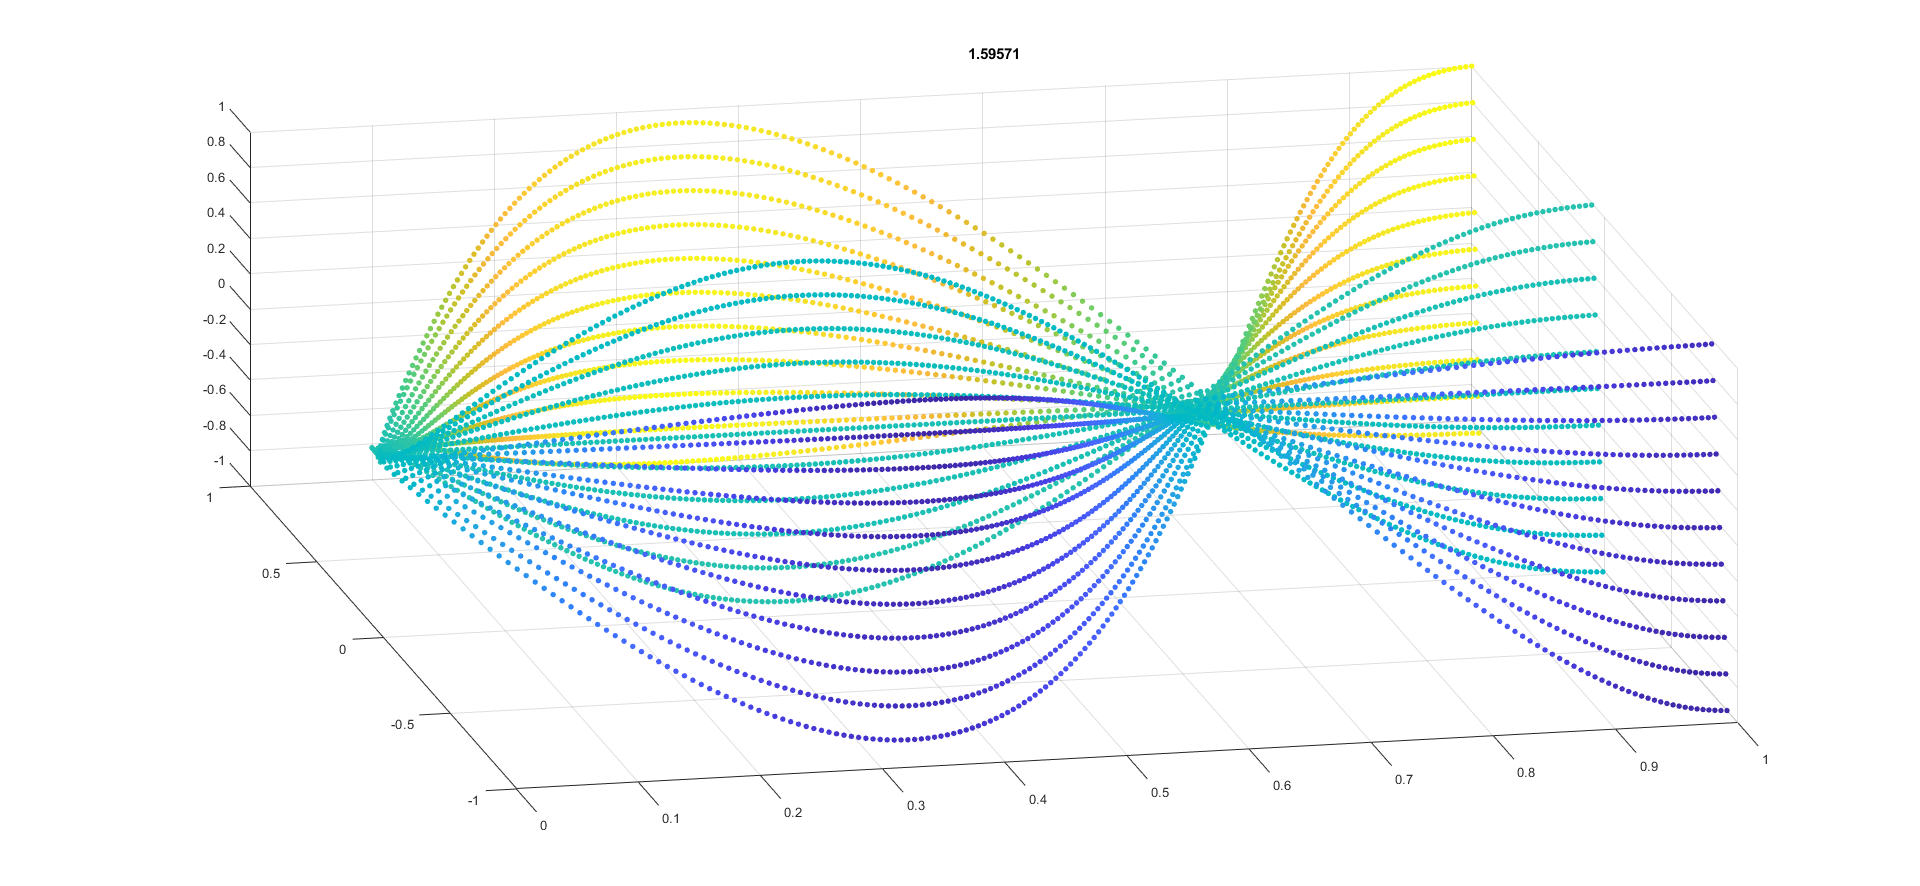
\includegraphics[width=1\linewidth]{3DNonBeam10.png}
				\subcaption{Non-2D Type - $\lambda_{10}$}
				\label{fig:minipage2}
			\end{minipage}
			\begin{minipage}[b]{0.8\linewidth}
				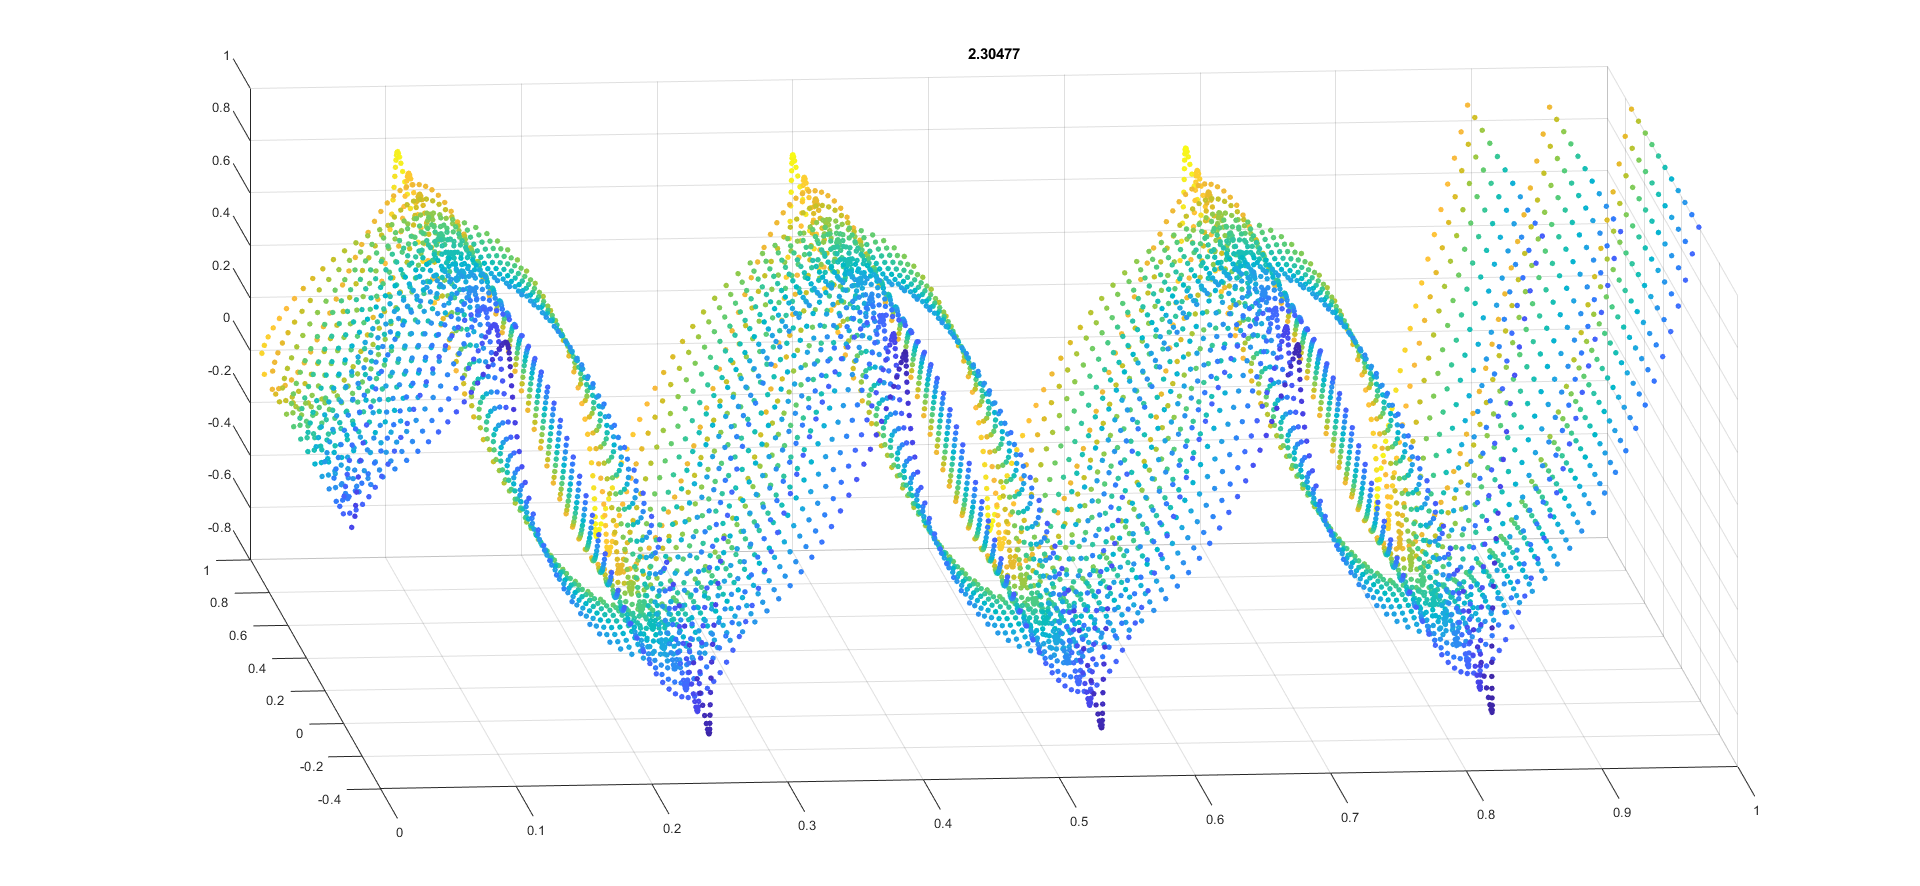
\includegraphics[width=1\linewidth]{3DNonBeam11.png}
				\subcaption{Non-2D Type - $\lambda_{11}$}
				\label{fig:minipage11}
			\end{minipage}
			\caption{Mode shapes of the displacement $w$ with $\alpha = 4800$.}
			
	}}
\end{figure}
\FloatBarrier

\subsection{Comparing the eigenvalues}
The eigenvalues of the two models can now be compared. Recall from the introduction, that the two-dimensional and three-dimensional models have different paramaters.

The two-dimensional model has the single parameter $h$ representing the height of the beam. The three-dimensional model has two parameters, $h$ and $b$, representing the height and width of the beam respectively. There are thus infinite possibilities for combinations of parameters that can be considered. However only a small number of combinations need to be considered to show that the two-dimensional model is a good approximation of the three-dimensional model.

For $h$, the values used in the previous section will be used. These values covers a range of beam shapes from a short fat beam, to a long slender beam with respect to the length to height ratio. For a short and fat beam, consider $h = 1/5$ and for a long and slender beam, consider $h = 1/20$.

For $b$, two different cases will be considered. The first case is for $b <= h$, and the $b>h$. Incremental increase/decrease of $b$ will then be used to compare the models.

In all of the tables to follow, the non-beam type eigenvalues that are not present in the two-dimensional model are omitted. The beam and non-beam type eigenvalues that both models share are included, with the non-beam type eigenvalues highlighted in grey.

\subsubsection*{Case $b < h$:}
Intuitively, for this case the two-dimensional model should be a good approximation of the three-dimensional model when considering the shape and definition of the two-dimensional model.

Table \ref{ab:2v3_1} below compares the eigenvalues of the models for a beam with a small length to height ratio of $h=1/5$ with decreasing values of $b$. 

\begin{table}[htbp]
	\scalebox{.8}{
	\makebox[\textwidth]{
		\caption{Comparsion of Eigenvalues with $h = 1/5$, with decreasing $b$ and $b < h$.}
		\begin{tabular}{|cc|cc|cc|cc||cc|}
			\hline
			\multicolumn{10}{|c|}{Eigenvalues} \\
			\hline
			\hline
			i     & {b = h} & i     & {b = 1/2 h} & i     & {b = 1/4 h} & i     & {b = 1/8 h} & j     & 2D \\
			\hline
			{2} & 0.12307 & {2} & 0.12234 & {2} & 0.12198 & {3} & 0.12178 & 1     & 0.12151 \\
			{3} & 3.5773 & {5} & 3.5630 & {6} & 3.5558 & {8} & 3.5519 & 2     & 3.5460 \\
			\rowcolor{lightgray}{5} & 7.7799 & {6} & 7.7596 & {8} & 7.7471 & {11} & 7.7401 & 3     & 7.7311 \\
			{8} & 20.334 & {9} & 20.283 & {11} & 20.26 & {14} & 20.247 & 4     & 20.225 \\
			{10} & 56.247 & {12} & 56.173 & {15} & 56.156 & {22} & 56.142 & 5     & 56.109 \\
			\rowcolor{lightgray}{11} & 69.197 & {14} & 69.319 & {17} & 69.281 & {24} & 69.238 & 6     & 69.164 \\
			{14} & 114.03 & {16} & 114.01 & {20} & 114.05 & {29} & 114.06 & 7     & 114.03 \\
			\rowcolor{lightgray}{17} & 187.01 & {19} & 189.14 & {25} & 189.37 & {36} & 189.34 & 8     & 189.17 \\
			{18} & 192.21 & {20} & 192.41 & {26} & 192.58 & {37} & 192.63 & 9     & 192.61 \\
			{21} & 284.76 & {23} & 285.43 & {31} & 285.74 & {42} & 285.84 & 10    & 285.85 \\
			{23} & 327.57 & {26} & 328.24 & {35} & 328.37 & {46} & 328.40 & 11    & 328.40 \\
			\rowcolor{lightgray}{25} & 347.77 & {28} & 356.44 & {36} & 357.30 & {50} & 357.33 & 12    & 357.08 \\
			{27} & 393.69 & {30} & 396.84 & {38} & 397.28 & {53} & 397.37 & 13    & 397.33 \\
			{30} & 434.46 & {34} & 441.05 & {41} & 441.81 & {57} & 441.99 & 14    & 442.00 \\
			\rowcolor{lightgray}{31} & 523.65 & {36} & 534.04 & {43} & 534.17 & {63} & 534.03 & 15    & 533.71 \\
			{34} & 550.51 & {37} & 537.82 & {44} & 538.86 & {64} & 539.06 & 16    & 538.97 \\
			\rowcolor{lightgray}{37} & 590.86 & {41} & 587.43 & {48} & 594.17 & {65} & 595.58 & 17    & 596.06 \\
			{39} & 590.86 & {42} & 600.52 & {49} & 602.25 & {67} & 602.69 & 18    & 602.77 \\
			\rowcolor{lightgray}{42} & 646.21 & {44} & 657.22 & {50} & 658.04 & {71} & 658.06 & 19    & 657.87 \\
			{44} & 711.07 & {46} & 714.62 & {53} & 717.10 & {73} & 717.51 & 20    & 717.37 \\
			\hline
			\hline
			\multicolumn{2}{|c|}{Max RE: \  2.6069\%} &\multicolumn{2}{c|}{Max RE: \ 1.4469\%}  & \multicolumn{2}{c|}{Max RE: \  0.38192\%}  & \multicolumn{2}{c||}{Max RE: \ 0.22301\%}& \multicolumn{2}{c|}{-} \\
			\hline
		\end{tabular}%
		\label{tab:2v3_1}%
	}}
\end{table}%
\FloatBarrier
Table \ref{tab:2v3_1} show that the two-dimensional modes compares well to the three-dimensional beam for $b<=h$. As the width decreases, the two-dimensional model becomes a better approximation of the three-dimensional model.

Table \ref{tab:2Dv3D_1_breakup} breaks up the maximum relative error for the beam type and non-beam type eigenvalues. The conclusion still holds.

% Table generated by Excel2LaTeX from sheet 'Sheet2'
\begin{table}[htbp]
	\centering
	\caption{Maximum relative error for beam type and non-beam type eigenvalues for $h = 1/5$.}
	\begin{tabular}{|c|cccc|}
		\hline
		\multicolumn{5}{|c|}{Maximum Relative Error} \\
		\hline
		\hline
		& {b = h} & {b = 1/2h} & {b = 1/4h} & {b = 1/8h} \\
		\hline
		Beam Type & 2.1420 \% & 0.6804 \% & 0.38192 \% & 0.22301 \% \\
		Non-Beam Type & 2.6069 \% & 1.4469 \% & 0.31546 \% & 0.11680 \% \\
		\hline
	\end{tabular}%
	\label{tab:2Dv3D_1_breakup}%
\end{table}%

Table \ref{tab:2v3_2} below is similar to Table \ref{tab:2v3_1} but compares the eigenvalues of the models for a beam with a large length to height ratio of $h=1/20$ with decreasing values of $b$. 

\begin{table}[ht]
	\scalebox{.8}{
	\makebox[\textwidth]{
	\caption{Comparsion of Eigenvalues with $h = 1/20$, with decreasing $b$ and $b < h$.}
	\begin{tabular}{|cc|cc|cc|cc||cc|}
		\hline
		\multicolumn{10}{|c|}{Eigenvalues} \\
		\hline
		\hline
		i     & {b = h} & i     & {b = 1/2 h} & i     & {b = 1/4 h} & i     & {b = 1/8 h} & j     & 2D \\
		\hline
		{2} & 0.008043 & {2} & 0.008029 & {2} & 0.008023 & {3} & 0.00802 & {1} & {0.008013} \\
		{3} & 0.3087 & {4} & 0.30816 & {5} & 0.30794 & {7} & 0.30785 & {2} & {0.30757} \\
		{5} & 2.3357 & {8} & 2.3316 & {9} & 2.3300  & {12} & 2.3293 & {3} & {2.3273} \\
		\rowcolor{lightgray}{8} & 7.7217 & {10} & 7.7156 & {13} & 7.7124 & {16} & 7.7111 & {4} & {7.7077} \\
		{10} & 8.5387 & {11} & 8.5238 & {14} & 8.5182 & {18} & 8.516 & {5} & {8.5086} \\
		{11} & 21.986 & {14} & 21.948 & {18} & 21.934 & {24} & 21.929 & {6} & {21.911} \\
		{14} & 45.863 & {18} & 45.781 & {21} & 45.756 & {30} & 45.746 & {7} & {45.712} \\
		\rowcolor{lightgray}{17} & 69.444 & {19} & 69.408 & {25} & 69.385 & {33} & 69.374 & {8} & {69.344} \\
		{18} & 83.149 & {22} & 82.999 & {27} & 82.960 & {36} & 82.944 & {9} & {82.887} \\
		{21} & 136.44 & {25} & 136.19 & {31} & 136.14 & {42} & 136.12 & {10} & {136.03} \\
		\rowcolor{lightgray}{23} & 192.62 & {27} & 192.62 & {35} & 192.58 & {47} & 192.56 & {11} & {192.48} \\
		{25} & 207.87 & {29} & 207.5 & {36} & 207.43 & {48} & 207.41 & {12} & {207.29} \\
		{27} & 299.14 & {33} & 298.63 & {41} & 298.56 & {55} & 298.53 & {13} & {298.38} \\
		\rowcolor{lightgray}{30} & 376.68 & {35} & 377.01 & {44} & 377.01 & {58} & 376.98 & {14} & {376.83} \\
		{31} & 411.58 & {37} & 410.89 & {46} & 410.83 & {61} & 410.81 & {15} & {410.63} \\
		{34} & 546.15 & {40} & 545.27 & {50} & 545.24 & {66} & 545.23 & {16} & {545.03} \\
		\rowcolor{lightgray}{37} & 620.77 & {42} & 622.02 & {53} & 622.19 & {69} & 622.18 & {17} & {621.95} \\
		{39} & 703.55 & {44} & 702.49 & {54} & 702.29 & {71} & 702.53 & {18} & {702.31} \\
		{42} & 884.27 & {47} & 883.02 & {59} & 883.14 & {82} & 883.19 & {19} & {882.96} \\
		\rowcolor{lightgray}{44} & 923.68 & {49} & 926.88 & {60} & 927.43 & {86} & 927.50 & {20} & {927.18} \\
		\hline
		\hline
		\multicolumn{2}{|c|}{Max RE: \  0.37701\%} &\multicolumn{2}{c|}{Max RE: \ 0.19893\%}  & \multicolumn{2}{c|}{Max RE: \  0.12393\%}  & \multicolumn{2}{c||}{Max RE: \ 0.092843\%}& \multicolumn{2}{c|}{-} \\
		\hline
	\end{tabular}%
	\label{tab:2v3_2}%
}}
\end{table}%
\FloatBarrier

Table \ref{tab:2v3_2} shows that the two-dimensional beam compares very well to the three-dimensional beam. For this long and slender beam, the two-dimensional model is an exellent approximation, and the approximation improves as the width $b$ decreases.

Table \ref{tab:2v3_2_split} breaks up the maximum relative error for the beam type and non-beam type eigenvalues. The conclusion still holds.

\begin{table}[htbp]
	\centering
	\caption{Maximum relative error for beam type and non-beam type eigenvalues for $h = 1/20$}
	\begin{tabular}{|c|cccc|}
		\hline
		\multicolumn{5}{|c|}{Maximum Relative Error} \\
		\hline
		\hline
		& {b = h} & {b = 1/2h} & {b = 1/4h} & {b = 1/8h} \\
		\hline
		Beam Type & 0.37701 \% & 0.19893 \% & 0.12393 \% & 0.092843 \% \\
		Non-Beam Type & 0.37682 \% & 0.10218 \% & 0.061213 \% & 0.043601 \% \\
		\hline
	\end{tabular}%
	\label{tab:2v3_2_split}%
\end{table}%
\FloatBarrier

From these results, it is clear that the two-dimensional model compares very well to the three-dimensional model for $b<=h$. The two-dimensional model is an excellent approximation for long and slender beams, and the approximation improves as the width $b$ decreases. 

For applications, very small values of the width $b$ are not always realistic, however the cases $b = h$ and $b=1/2h$ are realistic or close to realistic. And for these cases, the two-dimensional model still compare very well. 

\subsubsection*{Case $b > h$:}
In this section, the case where $b > h$ is investigated. Similar to the previous case, the two cases of $h = 1/5$ and $h = 1/20 $ are considered, and the width $b$ is increased incrementally.

\textcolor{red}{Results for $h = 1/5$}


In Table \ref{tab:b>h}, the height of the beam is set to $h=1/20$, which was the best case when $b<h$.

\FloatBarrier
\begin{table}[htbp]
	\scalebox{.8}{
	\makebox[\textwidth]{
		\caption{Comparsion of Eigenvalues with $h = 1/20$, with increasing $b$ and $b > h$}
		\begin{tabular}{|cc|cc|cc||cc|}
			\hline
			\multicolumn{8}{|c|}{Eigenvalues} \\
			\hline
			\hline
			i     & {b = 2h} & i     & {b = 4h} & i     & {b = 8h} & j     & 2D \\
			\hline
			{2} & 0.008076 & {1} & 0.008162 & {1} & 0.008324 & 1     & 0.008013 \\
			{3} & 0.30995 & {3} & 0.31298 & {3} & 0.31738 & 2     & 0.30757 \\
			{5} & 2.3462 & {5} & 2.3737 & {6} & 2.4116 & 3     & 2.3273 \\
			\rowcolor{lightgray}{8} & 7.7312 & {8} & 7.7471 & {9} & 7.7711 & 4     & 7.7077 \\
			{10} & 8.5841 & {9} & 8.7082 & {10} & 8.7929 & 5     & 8.5086 \\
			{11} & 22.124 & {12} & 22.491 & {14} & 23.222 & 6     & 21.911 \\
			{14} & 46.195 & {14} & 47.003 & {18} & 47.921 & 7     & 45.712 \\
			\rowcolor{lightgray}{17} & 69.454 & {17} & 69.281 & {22} & 72.307 & 8     & 69.344 \\
			{18} & 83.822 & {18} & 85.218 & {24} & 80.607 & 9     & 82.887 \\
			{21} & 137.43 & {21} & 138.58 & {32} & 140.97 & 10    & 136.03 \\
			\hline
			\hline
			\multicolumn{2}{|c|}{Max RE: \  1.1289\%} &\multicolumn{2}{c|}{Max RE: \ 2.8261\%}  & \multicolumn{2}{c|}{Max RE: \  5.9821\%} & \multicolumn{2}{c|}{-} \\
			\hline
		\end{tabular}%
		\label{tab:b>h}%
	}}
\end{table}
\FloatBarrier

In Table \ref{tab:b>h}, $h = 1/20$, it is clear that even the beams with a larger lenght to width ratio, the two-dimensional model compares less well to the three-dimensional model as $b$ increases.

Table \ref{tab:b>h-split}, again splits the beam and non-beam type maximum relative errors.

\FloatBarrier
\begin{table}[htbp]
	\centering
	\caption{Maximum relative error for beam type and non-beam type eigenvalues for $h = 1/20$}
	\begin{tabular}{|c|ccc|}
		\hline
		\multicolumn{4}{|c|}{Maximum Relative Error} \\
		\hline
		\hline
		& {b = 2h} & {b = 4h} & {b = 8h} \\
		\hline
		Beam Type & 1.1289 \% & 2.8261 \% & 5.9821 \% \\
		Non-Beam Type & 0.30521 \% & 0.51096 \% & 4.2734 \% \\
		\hline
	\end{tabular}%
	\label{tab:b>h-split}%
\end{table}%
\FloatBarrier

From these result it is clear the the two-dimensional beam compares less well to the three-dimensional beam if the width $b$ is `too much' larger than the height $h$.

Overall the results show that there are cases where the two-dimensional model compares very well to the three-dimensional model and can be used as a substitute. The best case is when the beam has a large length to height ratio, and the width is equal to less than the height. 

When the width gets larger than the height of the beam, the two-dimensional model starts to compare less well, and the comparison degrades as this difference increases further. 

For practical applications, when cantilever body has a larger width than height, the use of a beam model must be brought into question. A different model, like a plate model might be a better choice. In the next section, the validity of the Reissner-Mindlin plate mode is investigated using the same methodology used so far in this chapter, and in \cite{LVV09}.


\end{document}